%-------------------------
%big-picture
%(c) H.Buchmann FHNW 2008
%$Id$
%export TEXINPUTS=${HOME}/fhnw/edu/:${HOME}/fhnw/edu/tinL/config/latex:${HOME}/fhnw/edu/config//:
%-------------------------
\documentclass{beamer}
\usepackage{latex/beamer}
%---------------------
%local defines
%(c) H.Buchmann FHNW 2009
%$Id$
%---------------------
\newcommand{\target} {\beaglebone\xspace}
\newcommand{\targetS}{{\bf BBG}\xspace}
\newcommand{\host}   {{\em Host}\xspace}
\newcommand{\targetroot} {{\bf target-root}\xspace}
\newcommand{\kernel} {{\bf kernel}\xspace}
\renewcommand{\c}{{\bf C}\xspace}
\newcommand{\cpp}{{\bf C++}\xspace}
\newcommand{\posix}{{\bf POSIX}\xspace}

\input{/home/buchmann/latex/dirtree/dirtree.tex}

\title{Kernel}
\begin{document}

\frame{\titlepage}

\begin{frame}{Ziele}{Neuer \kernel auf \target}
 \begin{itemize}
  \item Download
  \item Setup
  \item Konfiguration
  \item Kompilation
  \item Installation
 \end{itemize}
\end{frame}

\section{The Big Picture}
\begin{frame}{The Big Picture}{grosses Projekt}
 \begin{description}
  \item[Gegeben] Eine grosse Anzahl {\em source} Files
  \item[Gesucht] ein einziger File: das {\Large Image}
  \item[L�sung] �hnlich wie in {\bf 4-devel} 
  \begin{itemize}
   \item Toolchain
   \item Makefile
  \end{itemize}
 \end{description}
\end{frame}

\begin{frame}{Die Schichten}
 \begin{center}
  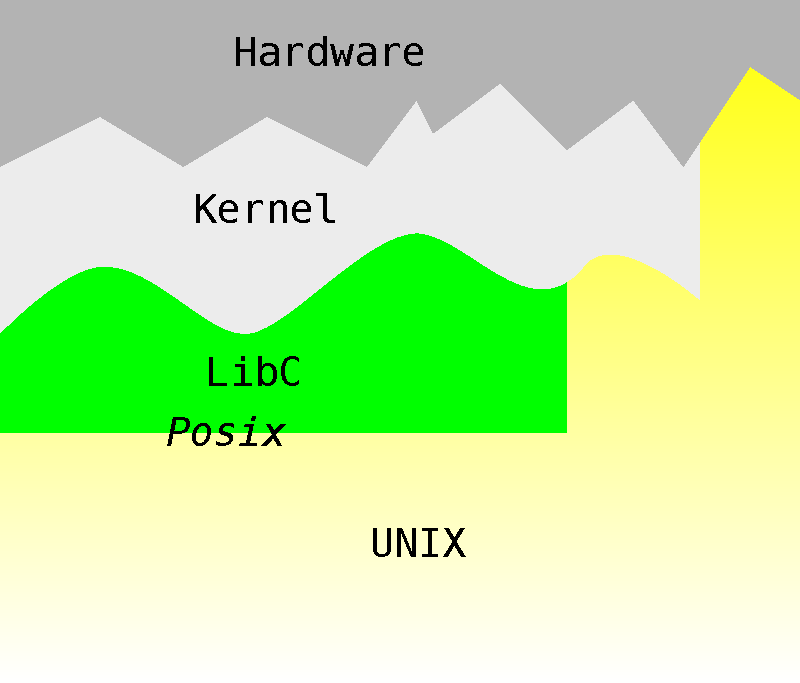
\includegraphics[width=0.75\textwidth]{layers.pdf}
 \end{center}
\end{frame}

\begin{frame}{Kernel}{Grosses Projekt}
\begin{block}{Was ist einfach ?}
 \begin{itemize}
  \item \kernel h�ngt nicht von anderen Software Komponenten ab
  \begin{itemize}
   \item stand alone
  \end{itemize}
  \item Braucht nur \cod{make} und {\em toolchain}
 \end{itemize}
\end{block}
\begin{block}{Was ist schwierig ?}
 \begin{itemize}
  \item Konfiguration
  \begin{itemize}
   \item Wahl der richtigen {\em source} Files f�r das {\Large Image}
  \end{itemize}
 \end{itemize}
\end{block}
\end{frame}

\section{Download}
\begin{frame}{\url{https://github.com/beagleboard/linux}}
             {Mehrere M�glichkeiten}
 \begin{itemize}
  \item das ganze git repository
  \item nur die letzten $n$ Versionen \cod{--depth=$n$}
  \item zip File 
 \end{itemize}
\end{frame}

\section{Setup}
\begin{frame}{Tools}{Siehe \cod{4-devel}}
 \begin{description}[toolchain]
 
  \item[toolchain] {\small \url{https://sourceforge.net/projects/fhnw-tinl/files}}
   \begin{itemize}
    \item \cod{beaglebone-black-toolchain-64bit.tar.bz2}
    \item Prefix: \cod{arm-linux-gnueabihf-}
    \begin{itemize}
     \item beschreibt:
     \begin{itemize}
      \item Architektur: \cod{armv7}
      \item {\bf A}pplication {\bf B}inary {\bf I}nterface: \cod{gnueabihf}
     \end{itemize}
    \end{itemize}
    \end{itemize}
  \item[make] Normales \cod{make}
  \begin{itemize}
   \item \kernel Herstellung:
   \begin{itemize}
    \item \cod{make {\em cmd}}
   \end{itemize}
  \end{itemize}
 \end{description}
\end{frame}

\begin{frame}{Wo ist was ?}
 \dirtree{%
  .1 tinL.
  .2 5-kernel.
  .3 build \DTcomment{generated kernel files}.
  .3 tools \DTcomment{for making}.
  .4 kernel.sh \DTcomment{wrapper to \kernel Makefile}.
  .3 config.
  .4 config.sh \DTcomment{for kernel.sh}.
  .2 resources.
  .3 beaglebone-black.
  .4 linux \DTcomment{the source tree}.
 }
\end{frame}

\section{Herstellung}
\begin{frame}{Konfiguration}{\cod{sh kernel.sh help}}
 \begin{itemize}
  \item \cod{sh tools/kernel.sh bb.org\_defconfig}
  \begin{itemize}
   \item Vordefinierte Konfiguration
  \end{itemize}
  \item \cod{sh tools/kernel.sh.sh menuconfig}
  \begin{itemize}
   \item Anpassung der Konfiguration
  \end{itemize}
 \end{itemize}
\end{frame}

\begin{frame}{Kompilation}
 \begin{itemize}
  \item \cod{sh tools/kernel.sh zImage}
  \begin{itemize}
   \item erzeugt  \cod{build/arch/arm/boot/zImage}
  \end{itemize} 
  \item \cod{sh tools/kernel.sh dtbs}
  \begin{itemize}
   \item erzeugt \cod{build/arch/arm/boot/dts/am335x-boneblack-wl1835mod.dtb}
   {\em Devicetree} 
   \remark{{\em Devicetree} sp�ter behandelt}
  \end{itemize} 
 \end{itemize}
\end{frame}

\begin{frame}{Installation}{auf SD-Card}
 \begin{itemize}
  \item Kopiere
  \begin{description}[Devicetree]
   \item[Image] \cod{build/arch/arm/boot/zImage}
   \item[Devicetree] \cod{build/arch/arm/boot/dts/am335x-boneblack.dtb}
  \end{description}
  auf
  \begin{itemize}
   \item SD-Card {\em boot-partition}
  \end{itemize}
 \end{itemize}
\end{frame}

\begin{frame}{Start}{auf \target}
 \begin{itemize}
  \item u-boot
  \begin{itemize}
   \item UART-USB Kabel
  \end{itemize}
  \begin{itemize}
   \item Befehle in \cod{scripts/u-boot.cmd}
  \end{itemize}
 \end{itemize}
\end{frame}

\begin{exercise}{\kernel}
 \begin{itemize}
  \item \target {\em default} Konfiguration
  \begin{itemize}
   \item herstellen
   \item auf SD-Karte
   \item ausprobieren
  \end{itemize}
  \item Die {\em default} Konfiguration �ndern
%  \item f�ge Treiber f�r WLAN hinzu
 \end{itemize}
\end{exercise}

\end{document}

